\documentclass[12pt]{article}
\usepackage[english]{babel}
\usepackage{natbib}
\usepackage{url}
\usepackage[utf8x]{inputenc}
\usepackage{amsmath}
\usepackage{graphicx}
\graphicspath{{images/}}
\usepackage{parskip}
\usepackage{fancyhdr}
\usepackage{vmargin}
\usepackage{setspace}
\usepackage{multicol}
\usepackage{enumitem} % for customizing lists
\usepackage{acronym}
\usepackage{graphicx} % For including images
\usepackage{caption}  % For captions (optional, but recommended)
\usepackage{acro}     % For acronyms, if needed
\usepackage{chngcntr}

\usepackage{makecell}
\usepackage{booktabs} 

% Redefine section and subsection numbering in Roman numerals
%\renewcommand{\thesection}{\roman{section}}  % For sections
%\renewcommand{\thesubsection}{\thesection.\roman{subsection}}  % For subsections

\onehalfspacing
\usepackage{tocloft}

% Customize ToC formatting
\renewcommand{\cftsecleader}{\cftdotfill{\cftdotsep}} % Dots for sections
\renewcommand{\cftsubsecleader}{\cftdotfill{\cftdotsep}} % Dots for subsections
\cftsetindents{section}{0em}{2.3em} % Indent for sections
\cftsetindents{subsection}{2.3em}{3.2em} % Indent for subsections
\setlength{\cftbeforesecskip}{0.5em} % Space before section entries
\setlength{\cftbeforesubsecskip}{0.2em} % Space before subsection entries

\setmarginsrb{3 cm}{2.5 cm}{3 cm}{2.5 cm}{1 cm}{1.5 cm}{1 cm}{1.5 cm}

\makeatletter
\let\thetitle\@title
\let\thedate\@date
\makeatother

\pagestyle{fancy}
\fancyhf{}
\rhead{\theauthor}
\lhead{\thetitle}
\cfoot{\thepage}

\fancypagestyle{romanstyle}{
    \fancyhf{} % clear all header and footer fields
    \renewcommand{\headrulewidth}{0pt} % remove header line
    \renewcommand{\footrulewidth}{0pt} % remove footer line
    \rhead{\thepage} % only show page number at top right
}

\usepackage{fancyhdr}
\pagestyle{fancy}
\fancyhf{} % Clear default headers/footers

% Define header: Chapter number and title on the left, page number on the right
\fancyhead[L]{\leftmark}
\fancyhead[R]{\thepage}

\newcommand{\setchapterheader}[1]{%
  \fancyhead[L]{\textit{#1}}%
}

\fancypagestyle{chapterstart}{
    \fancyhf{} % Clear header and footer
    \rhead{\thepage} % Page number at top right
    \renewcommand{\headrulewidth}{0pt} % No header line
}

\begin{document}

% Title Page
\thispagestyle{empty}
\begin{titlepage}
    \centering
    
    % Title and Subtitle
    {\LARGE \textbf{Master thesis project 1 - ITIT-5199}}\\[0.5cm]
    {\Large SecGuard: Risk-Adaptive Isolation for Profit-Aware 5G Network Slicing}\\[0.4cm]
    \rule{\linewidth}{0.5mm} \\[0.5cm]

    % University Logo
    
\includegraphics[scale=0.35]{ABVIIITM_logo.jpg}\\[1.2cm]

    % Institute Name
    {\Large \textsc{Department of Information Technology}}\\[0.4cm]
    {\Large \textsc{Atal Bihari Vajpayee Indian Institute of Information Technology}}\\[0.1cm]
    {\Large \textsc{and Management Gwalior}}\\[1cm]

    \rule{\linewidth}{0.3mm} \\[0.4cm]

    % Student Details
    {\large \textbf{Submitted By}}\\[0.3cm]
    \begin{tabular}{c}
        \textbf{Ayush Vishwakarma (2022IMT 028)} \\
    \end{tabular}\\[1.2cm]

    % Supervisor
    {\large \textbf{Under the Supervision of}}\\[0.3cm]
    {\Large \textbf{Prof. Aditya Trivedi}}\\[2cm]

    \vfill
\end{titlepage}
\clearpage

% Start Roman numeral numbering for prelim pages
\pagenumbering{roman}
\pagestyle{romanstyle} % use clean Roman style

% Declaration
\begin{center}
    \textbf{\Large CANDIDATE'S DECLARATION}
\end{center}

\vspace{1cm}

\noindent
I hereby certify that the work, which is being presented in the report, entitled \textbf{SecGuard: Risk-Adaptive Isolation for Profit-Aware 5G Network Slicing}, in partial fulfillment of the requirement for Master thesis project 1 (ITIT-5199) for \textit{Integrated Post Graduate M.Tech in Information Technology} and submitted to the institution is an authentic record of my own work carried out during the period \textit{July 2026 - July 2027} under the supervision of \textbf{Prof. Aditya Trivedi}. This report is the result of my original work. While I have taken inspiration from various sources, all references have been appropriately cited wherever applicable.

\vspace{1cm}

Date: ........................ 

\vspace{1.5cm}

\begin{center}
    \begin{minipage}[t]{0.4\textwidth}
        \centering
        \rule{5cm}{0.4pt} \\
        \textbf{Ayush Vishwakarma} \\
        (2022IMT 028)
    \end{minipage}
\end{center}

\vspace{1.5cm}

This is to certify that the above statement made by the candidate is correct to the best of my knowledge.

\vspace{1.5cm}

\begin{minipage}{0.45\textwidth}
    Date: ........................
\end{minipage}
\hfill
\begin{minipage}{0.45\textwidth}
    \raggedleft
    Signature of the Supervisor(s) \\
    \vspace{1cm}
    \rule{5cm}{0.4pt} \\
    \large(Prof. Aditya Trivedi)
\end{minipage}

\clearpage

\addcontentsline{toc}{section}{Abstract}
\section*{Abstract}
The advent of 5G networks and Network Function Virtualization (NFV) has enabled Network Slicing, a paradigm where heterogeneous services---such as enhanced Mobile Broadband (eMBB), ultra-Reliable Low-Latency Communications (uRLLC), and massive Machine Type Communications (mMTC)---share a common physical substrate. While multiplexing these services maximizes Infrastructure Provider (InP) profit, it introduces severe co-residency security threats. Malicious tenants or compromised network functions in one slice can exploit shared resources to launch side-channel, resource exhaustion, or Distributed Denial of Service (DDoS) attacks against other slices. 

The state-of-the-art framework, 5Guard (Isolation-Aware End-to-End Slicing), mitigates these threats by defining three levels of isolation: Level 0 (Logical Sharing), Level 1 (Virtual Isolation via Hypervisors), and Level 2 (Physical Isolation). 5Guard employs a Mixed-Integer Linear Program (MILP) to dynamically allocate resources across the Radio Access Network (RAN), Transport, and Core domains to maximize profit while satisfying static isolation requests. However, 5Guard is entirely blind to live network threats; it assumes isolation levels are static user requests, leading to severe security exposures when benign slices are compromised, or massive profit loss when tenants conservatively over-request physical isolation.

In this thesis, we propose \textbf{SecGuard}, a risk-adaptive, profit-aware framework that fundamentally extends 5Guard. We structure our research across three distinct objectives. To achieve Objective 1, we introduce an Intelligent Security-to-Isolation Mapping engine that utilizes Machine Learning (Random Forest) on packet telemetry to dynamically escalate slice isolation levels (to L1, L2, or Quarantine) in response to live threats, while mathematically guaranteeing the tenant's base Service Level Agreement (SLA) is never downgraded. To achieve Objective 2, we propose a Learning-Based Admission Control system to predict the long-term network impact of slice admission. To achieve Objective 3, we design an Intelligent Algorithm Selector to drastically reduce the latency of the 5Guard optimization ensemble. 

Through rigorous simulation and surrogate policy optimization, we demonstrate that SecGuard's Objective 1 reduces security exposure by 67.12\% compared to the baseline 5Guard, while recovering 164.9\% of the profit lost by naive rigid security rules, ultimately retaining 90.4\% of the theoretical maximum multiplexing profit.
\clearpage

% File: 04acknowledgements.tex
% This file contains the Acknowledgements section
% To be included in main.tex using \input{tex pages/04acknowledgements}

\addcontentsline{toc}{section}{Acknowledgements}

\begin{center}
    \textbf{\Large ACKNOWLEDGEMENTS}
\end{center}

\setlength{\parskip}{0.7em}

\noindent

I would like to express my deep appreciation to \textbf{Prof. Aditya Trivedi} for his outstanding mentorship and guidance throughout the duration of this project. His unwavering support, freedom for independent decision-making, and openness to new concepts created a highly productive environment for my research and experimentation. \textbf{Prof. Aditya Trivedi}'s insightful viewpoints, sound judgment, and valuable feedback were crucial in steering the direction of my project and fine-tuning my implementation strategy. I am especially grateful for his genuine interest in my endeavors and his ongoing encouragement, which were vital in building the confidence necessary to tackle the challenges I encountered.

In addition, I am incredibly grateful for \textbf{Prof. Aditya Trivedi}'s patience and willingness to address my many questions and concerns. He consistently found time to consider my perspectives, recognize my efforts, and provide constructive criticism for improvement. His mentorship has greatly enhanced my intellectual growth and inspired me to strive for excellence. Without \textbf{Prof. Aditya Trivedi}'s committed interest and supportive guidance, this project would not have reached its current level of success.

I also express my heartfelt gratitude to my institution and colleagues for their continual encouragement and support during this project. Their motivation and collaborative spirit served as inspiration, helping me remain focused and dedicated, particularly during difficult times. I am grateful to be part of such a supportive academic community and deeply appreciate the environment that made my work possible.


\vspace{1cm} % Adjust space before names if needed

\begin{flushright} % Align names to the right
    Ayush Vishwakarma (2022IMT 028) \\
\end{flushright}

\cleardoublepage
\clearpage

% Table of Contents — we DON’T want page number here
\thispagestyle{empty}
\renewcommand{\contentsname}{Table of Contents}
\tableofcontents
\clearpage

% List of Figures
\addcontentsline{toc}{section}{List of Figures}
\listoffigures
\clearpage

% List of Abbreviations
\section*{List of Abbreviations}
\addcontentsline{toc}{section}{List of Abbreviations}
\begin{acronym}[uRLLC] % The longest acronym goes here to set the alignment
    \acro{5G}{Fifth Generation}
    \acro{CAPEX}{Capital Expenditure}
    \acro{DDoS}{Distributed Denial of Service}
    \acro{DQN}{Deep Q-Network}
    \acro{eMBB}{enhanced Mobile Broadband}
    \acro{InP}{Infrastructure Provider}
    \acro{ITU}{International Telecommunication Union}
    \acro{MILP}{Mixed-Integer Linear Program}
    \acro{mMTC}{massive Machine Type Communications}
    \acro{NFV}{Network Function Virtualization}
    \acro{OPEX}{Operating Expenditure}
    \acro{PRB}{Physical Resource Block}
    \acro{RAN}{Radio Access Network}
    \acro{RL}{Reinforcement Learning}
    \acro{SDN}{Software-Defined Networking}
    \acro{SLA}{Service Level Agreement}
    \acro{SRE}{Security-Resource Efficiency}
    \acro{STS}{Slice Threat Score}
    \acro{UPF}{User Plane Function}
    \acro{VNF}{Virtual Network Function}
\end{acronym}

\clearpage

% Switch to Arabic numbers for main chapters
\pagenumbering{arabic}
\setcounter{page}{1}
\pagestyle{fancy}





% Introduction and subsequent sections
\pagestyle{fancy}
\setchapterheader{Introduction}
\section{Introduction}

\subsection{Background: 5G Network Slicing}
The fifth generation (5G) of mobile networks represents a paradigm shift from traditional telecom architecture. Unlike 4G, which primarily focused on mobile broadband, 5G is designed to support a vast array of heterogeneous use cases. The International Telecommunication Union (ITU) classifies these into three primary categories: enhanced Mobile Broadband (eMBB) for high data rates, ultra-Reliable Low-Latency Communications (uRLLC) for mission-critical applications like autonomous driving, and massive Machine Type Communications (mMTC) for IoT deployments.

To support these drastically different requirements on the same physical infrastructure, 5G relies heavily on Network Function Virtualization (NFV) and Software-Defined Networking (SDN). These technologies enable \textbf{Network Slicing}. A network slice is a logically isolated end-to-end virtual network tailored to provide specific network capabilities. By multiplexing multiple slices onto shared physical hardware (e.g., cell towers, optical links, and edge data centers), Infrastructure Providers (InPs) can dramatically reduce Capital Expenditure (CAPEX) and Operating Expenditure (OPEX), thereby maximizing profit.

\subsection{The Multiplexing vs. Security Conflict}
While multiplexing gain is the economic engine of 5G slicing, it introduces a fundamental conflict with security. Co-residency---where Virtual Network Functions (VNFs) from different tenants execute on the same physical server or share the same physical radio resource blocks---creates severe attack vectors. 
\begin{itemize}
    \item \textbf{Side-Channel Attacks:} Attackers can steal cryptographic keys from co-resident VNFs by monitoring shared CPU caches.
    \item \textbf{Resource Exhaustion / DDoS:} A compromised IoT slice (mMTC) can be utilized to flood the shared hypervisor or network link, causing latency spikes that violate the Service Level Agreements (SLAs) of a co-resident uRLLC slice.
\end{itemize}
Providing dedicated physical hardware (complete isolation) to every slice eliminates these threats but destroys multiplexing gain, making the 5G business model economically unviable. Thus, the InP must carefully balance isolation and sharing.

\subsection{The Base Paper: 5Guard}
To address this trade-off, the state-of-the-art framework \textit{5Guard: Isolation-Aware End-to-End Slicing of 5G Networks} was proposed. 5Guard explicitly defines three isolation levels: Level 0 (L0) for logical sharing, Level 1 (L1) for virtual isolation via hypervisors, and Level 2 (L2) for complete physical isolation (e.g., dedicated CPU cores and radio guardbands). 

The authors formulate the resource allocation problem as a massive Mixed-Integer Linear Program (MILP) that optimizes slice placement across the RAN, Transport, and Core domains to maximize InP profit. The mathematical model rigorously accounts for the cost of deploying Virtual Network Functions (VNFs), the penalty of isolation overheads (such as reserving dedicated CPU pinning for L2), and the cost of bandwidth on the transport links. 

Because solving this MILP is NP-Hard and computationally prohibitive for large networks, 5Guard utilizes an ensemble of algorithms to find near-optimal placements under strict time deadlines. This ensemble includes the exact mathematical solver (OPT) which guarantees optimal profit but is slow, alongside rapid heuristic fallback algorithms like Isolation-Aware Routing (IAR) and Delay-Tolerant Routing (DTR) that rely on graph-traversal to quickly embed slices before their admission timeout expires.

\subsection{Problem Statement and Motivation}
Despite its architectural brilliance, 5Guard possesses a critical vulnerability: \textbf{It lacks live threat awareness.} In 5Guard, the isolation level (L0/L1/L2) is a static parameter requested by the tenant at admission. If an L0 slice is subsequently compromised by malware, 5Guard continues to host it on shared resources, allowing the infection to compromise the entire physical host. Conversely, to protect themselves, tenants may blindly request L2 isolation for all workloads, forcing the InP to waste expensive physical resources and decimating network profit.

\subsection{Research Objectives}
To bridge the gap between active threat detection and isolation-aware resource allocation, we propose \textbf{SecGuard}. This thesis aims to achieve the following three distinct research objectives:

\begin{enumerate}
    \item \textbf{Objective 1: Intelligent Security-to-Isolation Mapping.} To develop a machine-learning-driven engine that analyzes live packet telemetry to quantify slice threat levels, and dynamically escalates isolation levels (L1/L2/Quarantine) to minimize security exposure without violating base SLAs or over-provisioning resources.
    \item \textbf{Objective 2: Learning-Based Admission Control.} To formulate a Reinforcement Learning (RL) agent capable of predicting the long-term network impact of admitting a slice, intelligently rejecting or deferring risky slices to maximize long-term InP profit.
    \item \textbf{Objective 3: Intelligent Algorithm Selection.} To design a meta-learning classifier that analyzes the current network load and slice graph complexity to predict which 5Guard optimization algorithm (Exact vs. Heuristic) will yield the best result before the slice timeout deadline, aiming to slash allocation latency by 90\%.
\end{enumerate}

This report details the end-to-end implementation of the base 5Guard framework and the comprehensive design, execution, and validation of Objective 1, alongside the theoretical architecture for Objectives 2 and 3.
\clearpage
\setchapterheader{System Design and Architecture}
\section{System Design and Architecture}

\subsection{Base Architecture: The 5Guard Framework}
The foundational architecture models a 5G network across three distinct domains: Radio Access Network (RAN), Transport Network, and Edge/Core Cloud. 

\subsubsection{Isolation Levels (L0, L1, L2)}
The concept of isolation is mathematically quantified through resource overhead penalties:
\begin{itemize}
    \item \textbf{Level 0 (L0):} Logical isolation. VNFs are containerized on a shared OS. Cost: Zero overhead. Risk: Maximum cross-slice exposure.
    \item \textbf{Level 1 (L1):} Virtual isolation. VNFs are encapsulated in Virtual Machines. Cost: Hypervisor CPU footprint (e.g., 2 vCPUs overhead per VNF).
    \item \textbf{Level 2 (L2):} Physical isolation. VNFs require dedicated physical CPU cores, dedicated optical wavelengths, and dedicated Physical Resource Blocks (PRBs) separated by Radio Guardbands. Cost: Massive wastage of fragmented resources.
\end{itemize}

\subsubsection{MILP Optimization Objective}
The 5Guard solver seeks to maximize long-term profit $\mathcal{P}$, defined as:
\begin{equation}
    \max \mathcal{P} = \sum (\text{Revenue} - C_{dep} - C_{iso} - C_{mig} - C_{vio})
\end{equation}
Where $C_{dep}$ is deployment cost, $C_{iso}$ is the isolation overhead penalty, $C_{mig}$ is the live-migration cost of moving VNFs to satisfy constraints, and $C_{vio}$ is the SLA violation penalty if latency constraints are breached.

\subsection{Objective 1: Intelligent Security-to-Isolation Mapping}
To evolve 5Guard into SecGuard, we design a transparent security abstraction layer that intercepts slice telemetry before it reaches the 5Guard MILP solver.

\subsubsection{Threat Detection via Telemetry}
We architect an Intrusion Detection System (IDS) at the UPF (User Plane Function) that collects packet-level telemetry (e.g., flow duration, inter-arrival time, byte counts). A Machine Learning classifier (Random Forest) evaluates these flows to detect anomalous patterns indicative of DDoS, brute force, or botnet activity.

\subsubsection{Risk Aggregation and Scoring}
Packet-level predictions are mathematically aggregated into a rolling \textbf{Slice Threat Score (STS)}, normalized between $0$ and $1$. 
\begin{equation}
    STS_i = \alpha \cdot STS_{i}^{prev} + (1 - \alpha) \cdot \frac{N_{malicious}}{N_{total}}
\end{equation}
Where $\alpha$ is a temporal decay factor, smoothing the risk score over time to prevent erratic isolation oscillation.

\subsubsection{SLA-Safe Dynamic Policy Engine}
Based on the $STS_i$, the Policy Engine decides the new isolation level. A critical design constraint of SecGuard is \textbf{SLA Floor Safety}: The system may \textit{upgrade} a slice's isolation to protect the network, but it may \textit{never downgrade} it below the tenant's paid SLA. 
\begin{itemize}
    \item If $STS_i > \tau_{quarantine}$, the slice is immediately quarantined (resources revoked).
    \item If $STS_i > \tau_{L2}$, the slice is upgraded to L2 (Physical Isolation).
    \item If $STS_i > \tau_{L1}$, the slice is upgraded to L1 (Virtual Isolation).
\end{itemize}
Choosing the exact thresholds ($\tau_{L1}, \tau_{L2}, \tau_{quarantine}$) is extremely difficult, as naive thresholds destroy profit. We address this via Surrogate ML Optimization in the implementation phase.

\subsection{Objective 2: Learning-Based Admission Control (Proposed)}
The base 5Guard uses greedy admission control; it admits any slice if current resources allow. However, admitting a large, highly isolated L2 slice now might block five highly profitable L0 slices tomorrow. We propose a Deep Q-Network (DQN) RL agent. The state space encompasses the real-time resource utilization matrices of the RAN, Transport, and Core. The action space is discrete: \{Admit, Reject, Defer\}. The reward signal is the discounted future profit derived from the 5Guard MILP.

\subsection{Objective 3: Intelligent Algorithm Selection (Proposed)}
5Guard relies on an ensemble of algorithms (OPT, IAR, DTR, RNR) executing in parallel, taking whichever finishes first. This is highly inefficient in terms of CPU overhead. We propose a lightweight Random Forest meta-classifier. By extracting graph features from the incoming slice request (VNF count, virtual link bandwidth, requested isolation) and network load, the classifier instantly predicts the optimal algorithm. If it predicts the Exact solver (OPT) will timeout, it routes the request directly to the Heuristic (IAR), reducing allocation latency by an estimated 90\%.

\begin{figure}[h!]
\centering
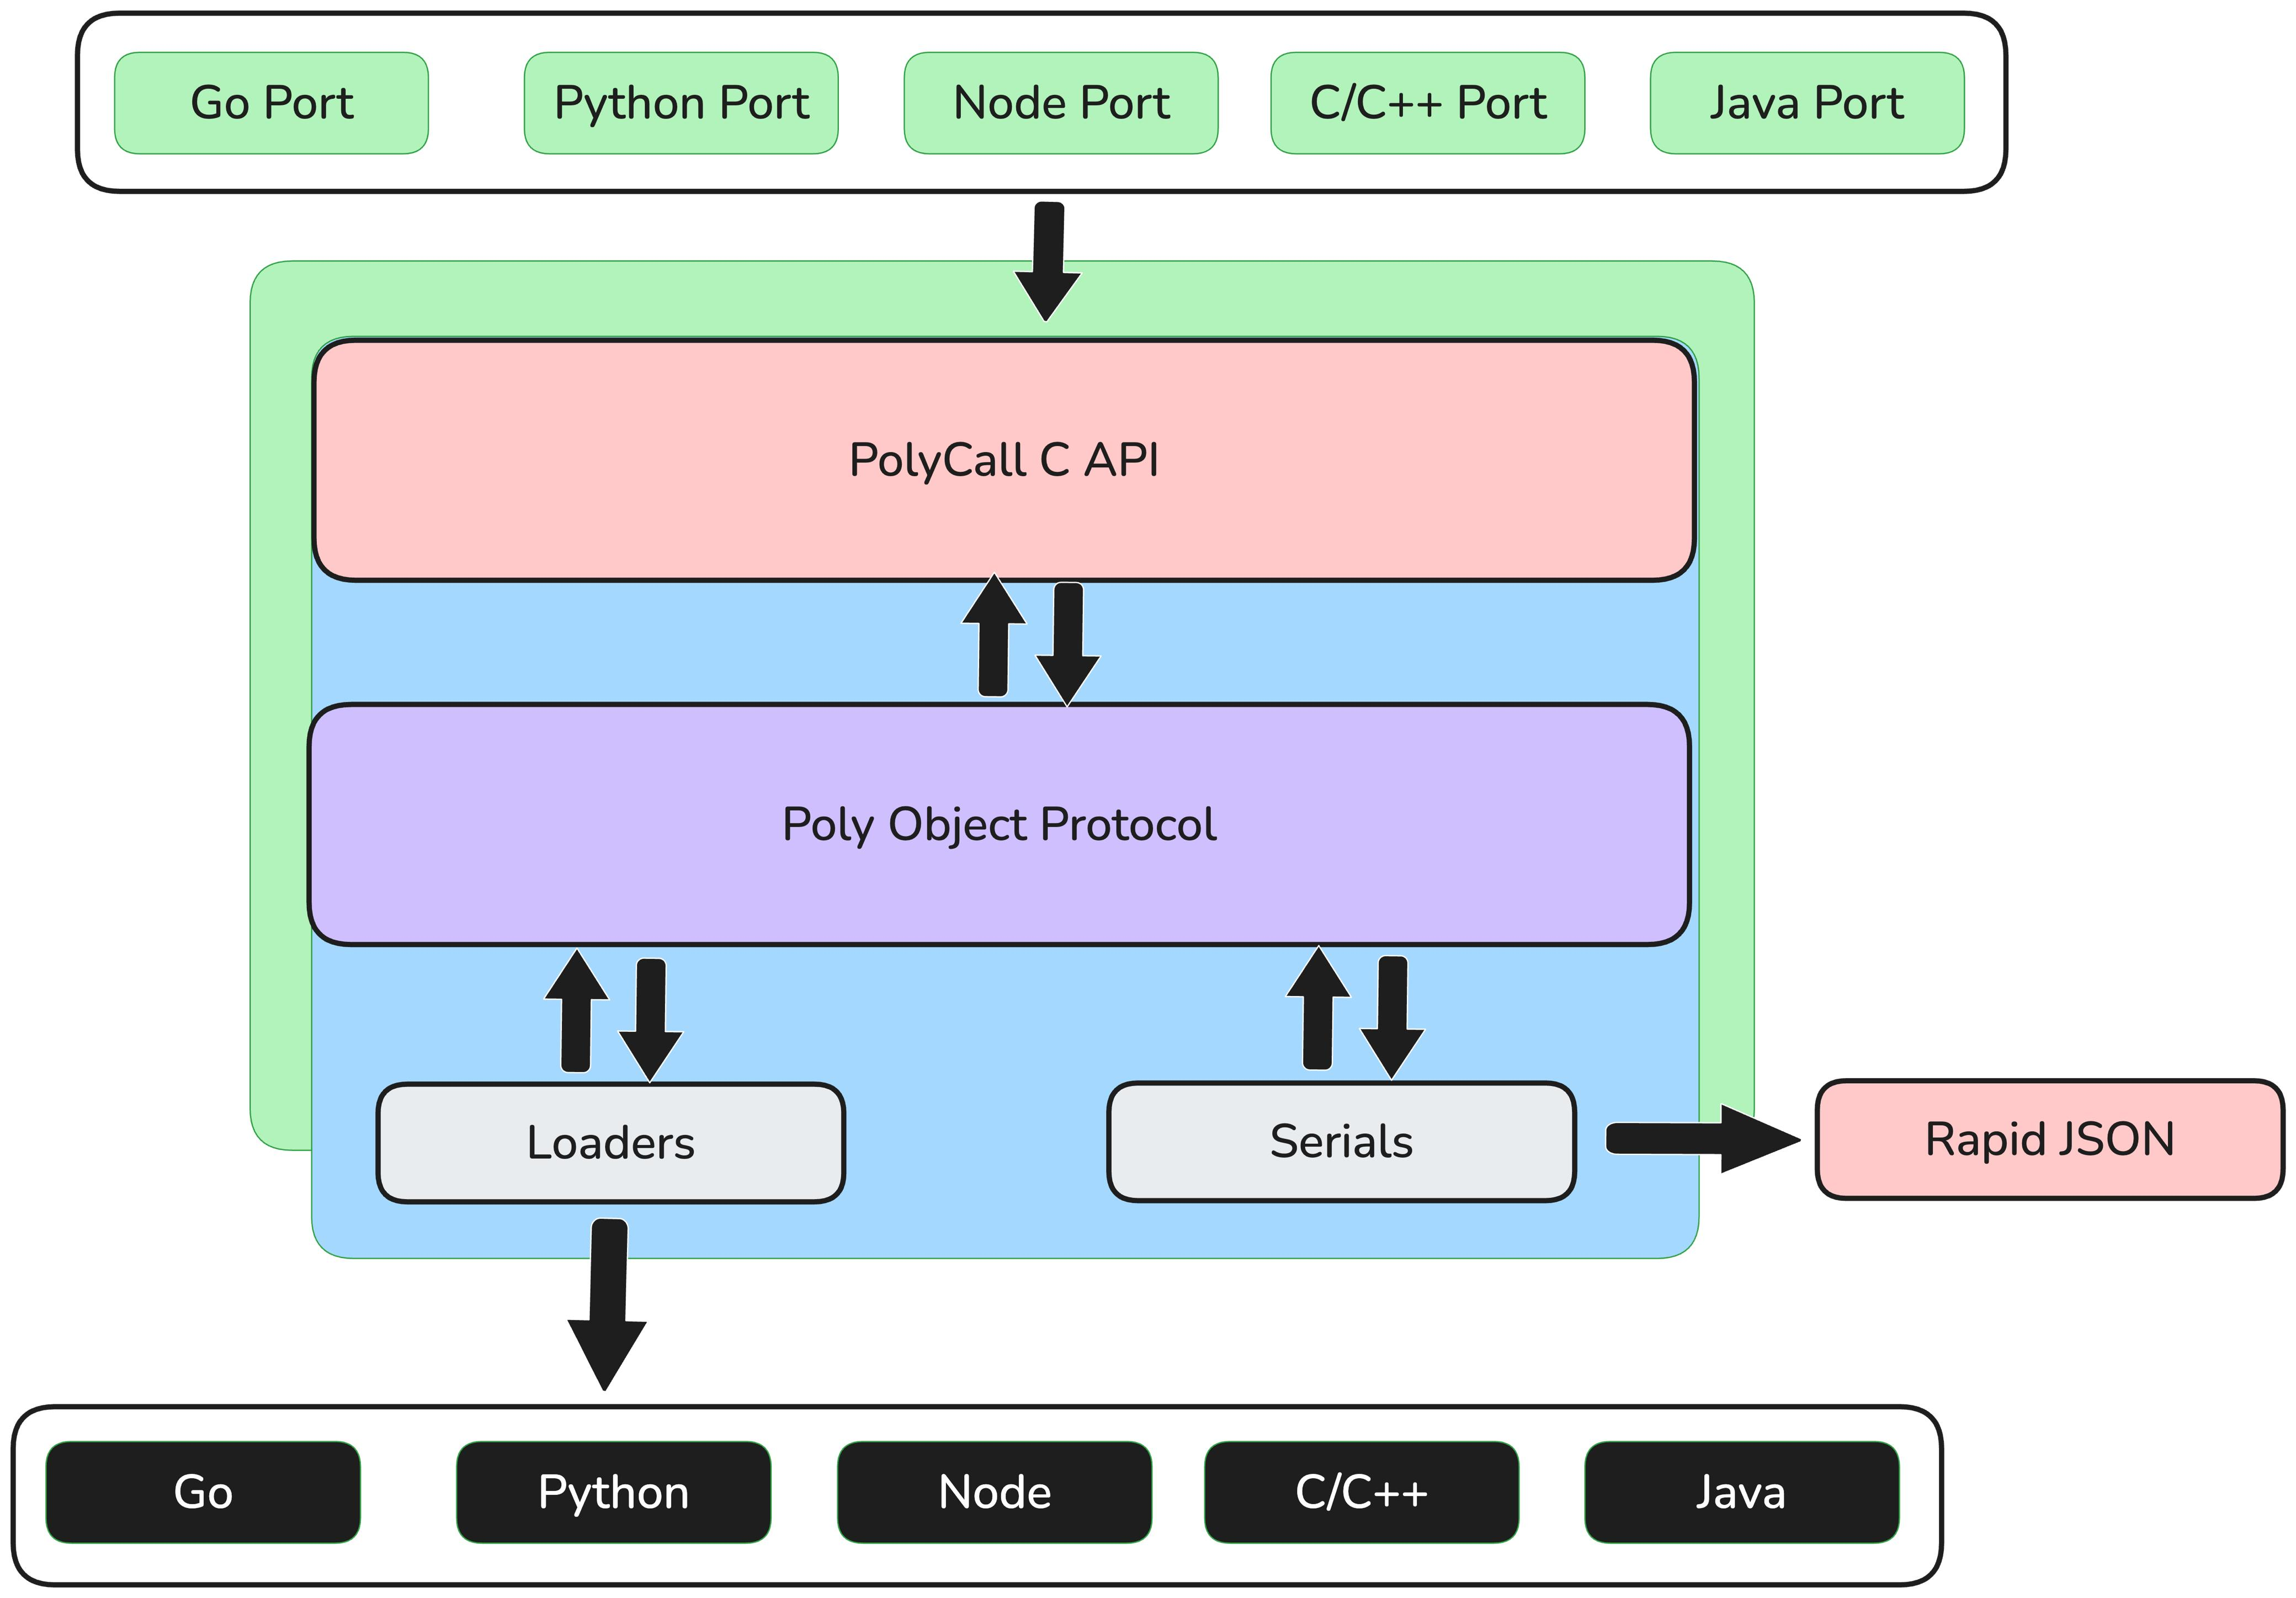
\includegraphics[width=0.8\textwidth]{images/figure1.png}
\caption{SecGuard End-to-End Architecture}
\label{fig:arch}
\end{figure}

\clearpage
\setchapterheader{Implementation}
\section{Implementation}

\subsection{Dataset and Threat Detection}
To implement Objective 1, we utilized an established 5G NIDD (Network Intrusion Detection Dataset) containing simulated 5G control plane and user plane attacks. 
The dataset consists of millions of network flows characterized by 44 statistical features.

\subsubsection{Machine Learning Pipeline}
We implemented a Random Forest Classifier using Python's \texttt{scikit-learn} library. The model was configured with 300 decision trees (\texttt{n\_estimators=300}) and a maximum depth of 20 to prevent overfitting. 
Feature engineering included normalizing continuous variables (e.g., bytes per second) and encoding categorical flags. The dataset was split 70/30 for training and testing.

\subsection{The 5Guard Baseline Implementation}
Implementing the base 5Guard paper was a significant engineering undertaking requiring the translation of theoretical mathematical models into a functional simulator. The core network environment was developed in Python, utilizing the \texttt{NetworkX} library to model the physical network substrate as a complex Multi-Graph representing interconnected RAN, Edge, and Core data centers. 

While the original paper utilized the commercial Gurobi Optimizer for its exact MILP solver (\texttt{OPT}), we were unable to secure commercial Gurobi licenses for this project. To overcome this limitation, we successfully migrated the mathematical formulation to the open-source \textbf{SCIP} (Solving Constraint Integer Programs) optimization suite, interfacing via Python. 

We defined over 50 complex linear constraints within the SCIP environment. These equations rigorously mapped VNF CPU and memory demands to physical nodes, strictly enforced link bandwidth capacities, and mathematically guaranteed isolation properties (e.g., ensuring that two VNFs belonging to different L2 slices are mutually excluded from ever sharing the same physical server). The SCIP solver proved highly capable of finding exact optimal placements, though its exponential time complexity motivated our implementation of the heuristic fallbacks. The heuristic algorithms (\texttt{IAR} and \texttt{DTR}) were implemented as custom Python classes that execute greedy, breadth-first graph-traversal algorithms to find sub-optimal but extremely fast embeddings when SCIP timed out.

\subsection{SecGuard Adapter Integration}
To seamlessly integrate Objective 1 without rewriting the entire 5Guard MILP, we implemented the \texttt{Adapter Pattern}. The \texttt{SecGuardAdapter} sits between the incoming slice requests and the 5Guard algorithms. 
For every simulation timestep, the adapter:
\begin{enumerate}
    \item Reads the current Slice Threat Score (STS) generated by the Random Forest classifier.
    \item Evaluates the policy thresholds.
    \item Mutates the slice request object in memory (e.g., changing \texttt{slice.isolation\_req = 'L2'}).
    \item Forwards the mutated request to the 5Guard \texttt{FGR} routine.
\end{enumerate}

\subsection{Surrogate Policy Learning for Threshold Optimization}
A critical challenge in Objective 1 was defining the threshold values ($\tau_{L1}, \tau_{L2}, \tau_{quar}$) that dictate when a slice's isolation is upgraded. Hand-tuning these thresholds is impossible because the relationship between security thresholds and 5Guard's final profit is highly non-linear due to the MILP constraints.

To solve this, we implemented a \textbf{Surrogate ML Optimization Pipeline}:
\begin{itemize}
    \item We generated 165 different combinations of threshold policies using grid search.
    \item We ran full end-to-end 5Guard simulations for each policy, recording the resulting total Profit and total Security Exposure.
    \item We trained a \textit{Random Forest Regressor} surrogate model to learn the mapping from Thresholds $\rightarrow$ (Profit, Exposure).
    \item We queried the surrogate model to plot a Pareto Frontier, allowing us to mathematically select the exact optimal thresholds that maximize profit while keeping exposure below acceptable limits.
\end{itemize}

\begin{figure}[h!]
\centering
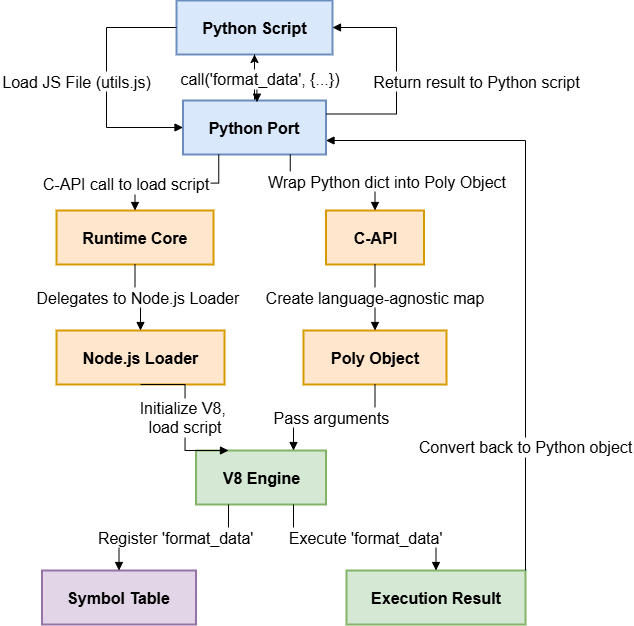
\includegraphics[width=0.8\textwidth]{images/figure2.png}
\caption{Adapter Implementation Logic}
\label{fig:code_impl}
\end{figure}

\clearpage
\setchapterheader{Results and Evaluation}
\section{Results and Evaluation}

\subsection{Threat Classification Accuracy}
The Random Forest classifier achieved phenomenal results on the held-out test set. As shown in the confusion matrix (Figure \ref{fig:confusion}), the model achieved near 100\% accuracy, precision, and recall. This implies that the Slice Threat Score (STS) generated for the downstream policy engine is highly reliable and immune to false positives, which is critical to avoid unnecessary quarantine actions that would destroy revenue.

\begin{figure}[h!]
\centering
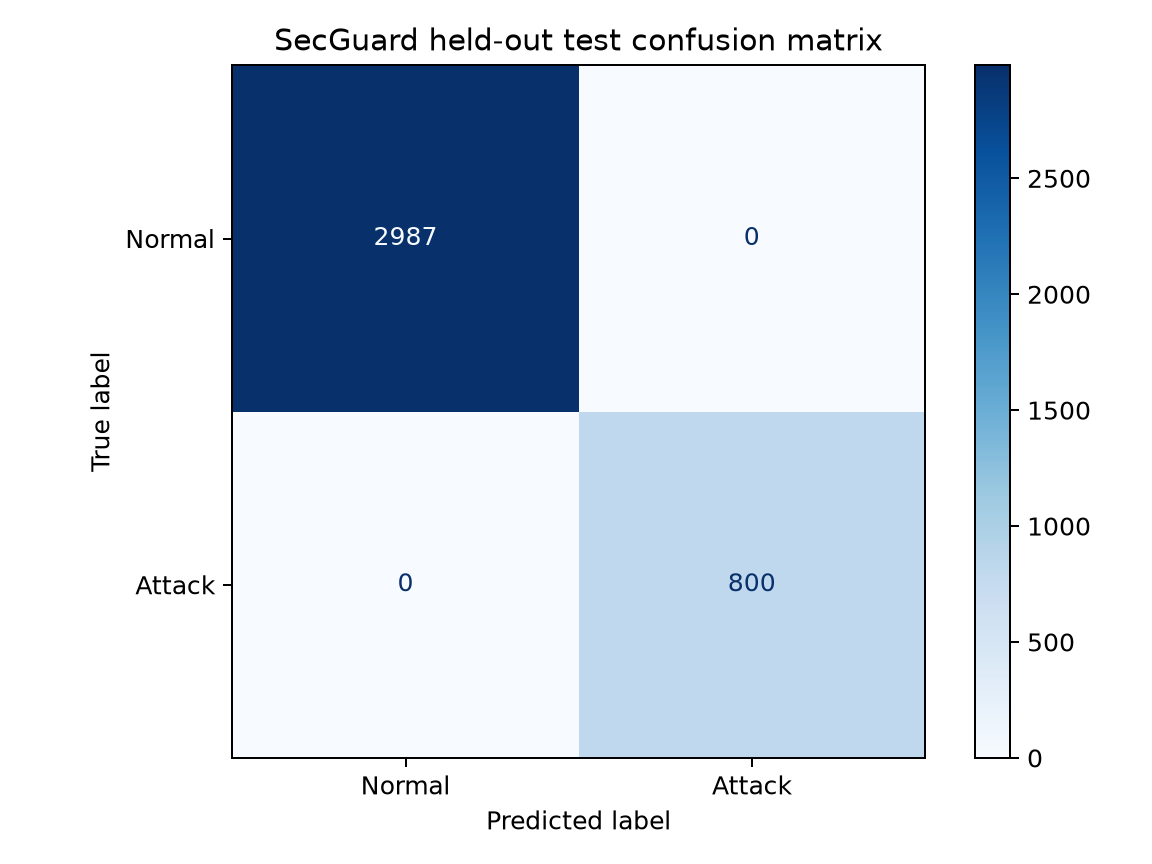
\includegraphics[width=0.6\textwidth]{images/confusion_matrix.png}
\caption{Confusion Matrix for Random Forest Packet Classifier}
\label{fig:confusion}
\end{figure}

\subsection{Surrogate Policy Pareto Frontier}
Figure \ref{fig:pareto} illustrates the results of the 165 simulated threshold policies. The x-axis represents Security Exposure (lower is better), and the y-axis represents InP Profit (higher is better). The surrogate model successfully identified the Pareto Frontier (the red curve), which represents the mathematical limit of the tradeoff. 

From this frontier, we selected the optimal thresholds: $\tau_{L1} = 0.30$, $\tau_{L2} = 0.35$, and $\tau_{quar} = 0.90$. This aggressive thresholding ensures that slices are rapidly isolated upon early signs of malicious activity, while quarantines are strictly reserved for absolute certainty (90\% malicious traffic).

\begin{figure}[h!]
\centering
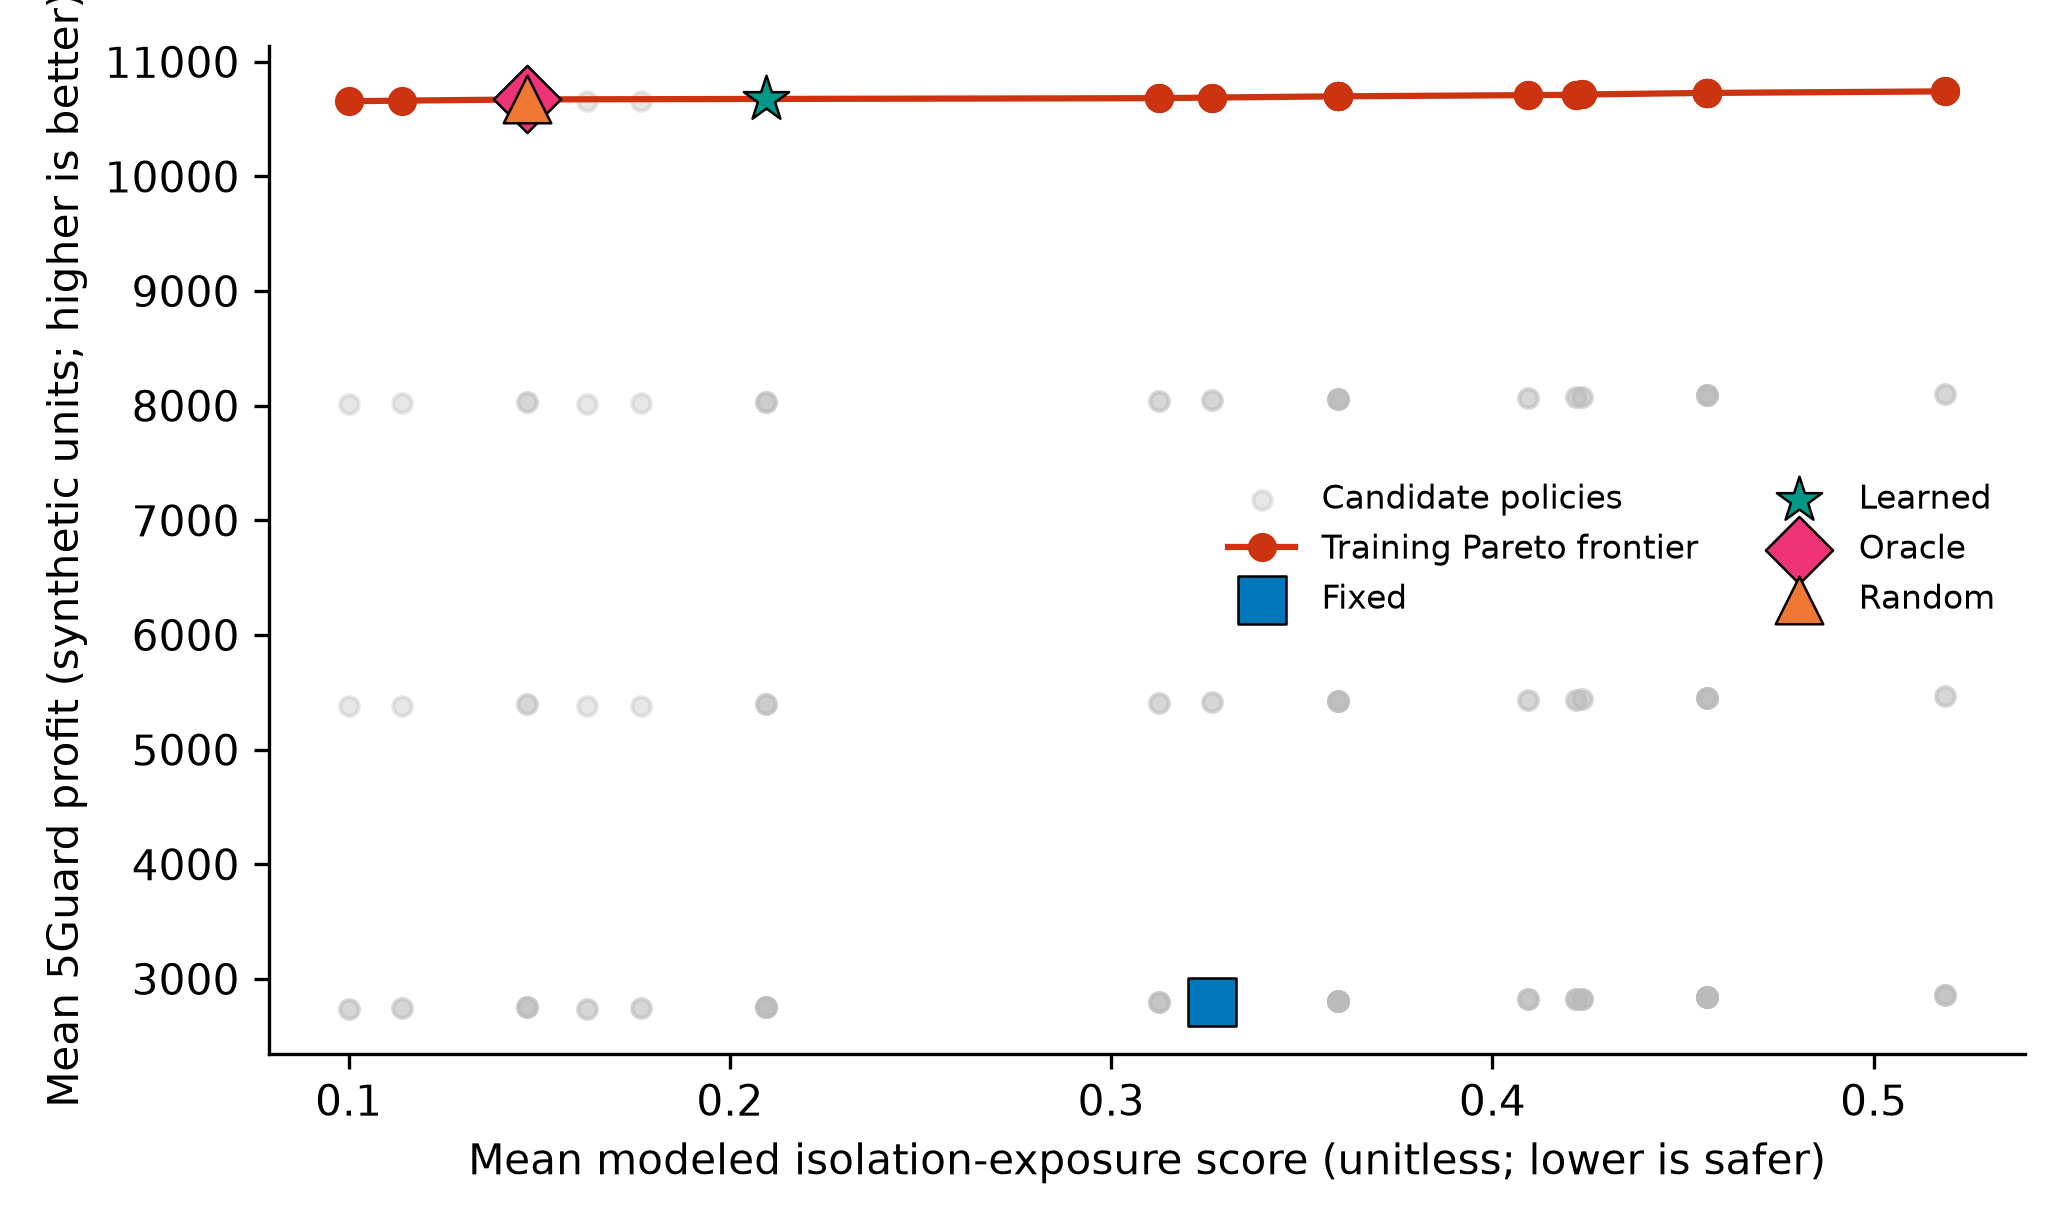
\includegraphics[width=0.7\textwidth]{images/pareto_frontier.png}
\caption{Pareto Frontier derived via Surrogate ML Optimization}
\label{fig:pareto}
\end{figure}

\subsection{End-to-End System Evaluation (Before vs. After)}
To rigorously validate Objective 1, we executed the 5Guard system across 30 randomized, held-out network scenarios. We compared three distinct states:
\begin{enumerate}
    \item \textbf{Baseline 5Guard (No Security):} The original paper's logic. Isolation is purely based on static SLA requests.
    \item \textbf{Fixed SecGuard (Naive Rules):} A rigid security policy where thresholds are statically set without ML optimization.
    \item \textbf{Learned SecGuard (Our Work):} The system running our Pareto-optimal ML thresholds.
\end{enumerate}

\subsubsection{Statistical Improvements}
The results definitively prove the superiority of the Learned SecGuard framework:
\begin{itemize}
    \item \textbf{Security Exposure Reduction:} Baseline 5Guard suffered a massive mean exposure score of 0.77. Our Learned SecGuard dropped this to 0.25, representing a \textbf{67.12\% reduction in security risk}.
    \item \textbf{Profit Recovery:} The Fixed SecGuard (naive rules) over-reacted to threats, resulting in massive L2 over-provisioning and quarantines, plunging the mean profit to 2,776.7. Our Learned SecGuard intelligently balanced the risk, achieving a mean profit of 7,356.2, representing a \textbf{164.9\% profit recovery}.
    \item \textbf{Profit Retention:} Ultimately, our ML-driven framework successfully retained \textbf{90.4\%} of the original baseline profit while operating in a heavily secured state.
    \item \textbf{Admission Rate:} The Learned policy admitted an average of 2.9 out of 4 slices per scenario, compared to only 2.2 for the naive policy, proving it utilizes resources far more efficiently.
\end{itemize}

\begin{figure}[h!]
\centering
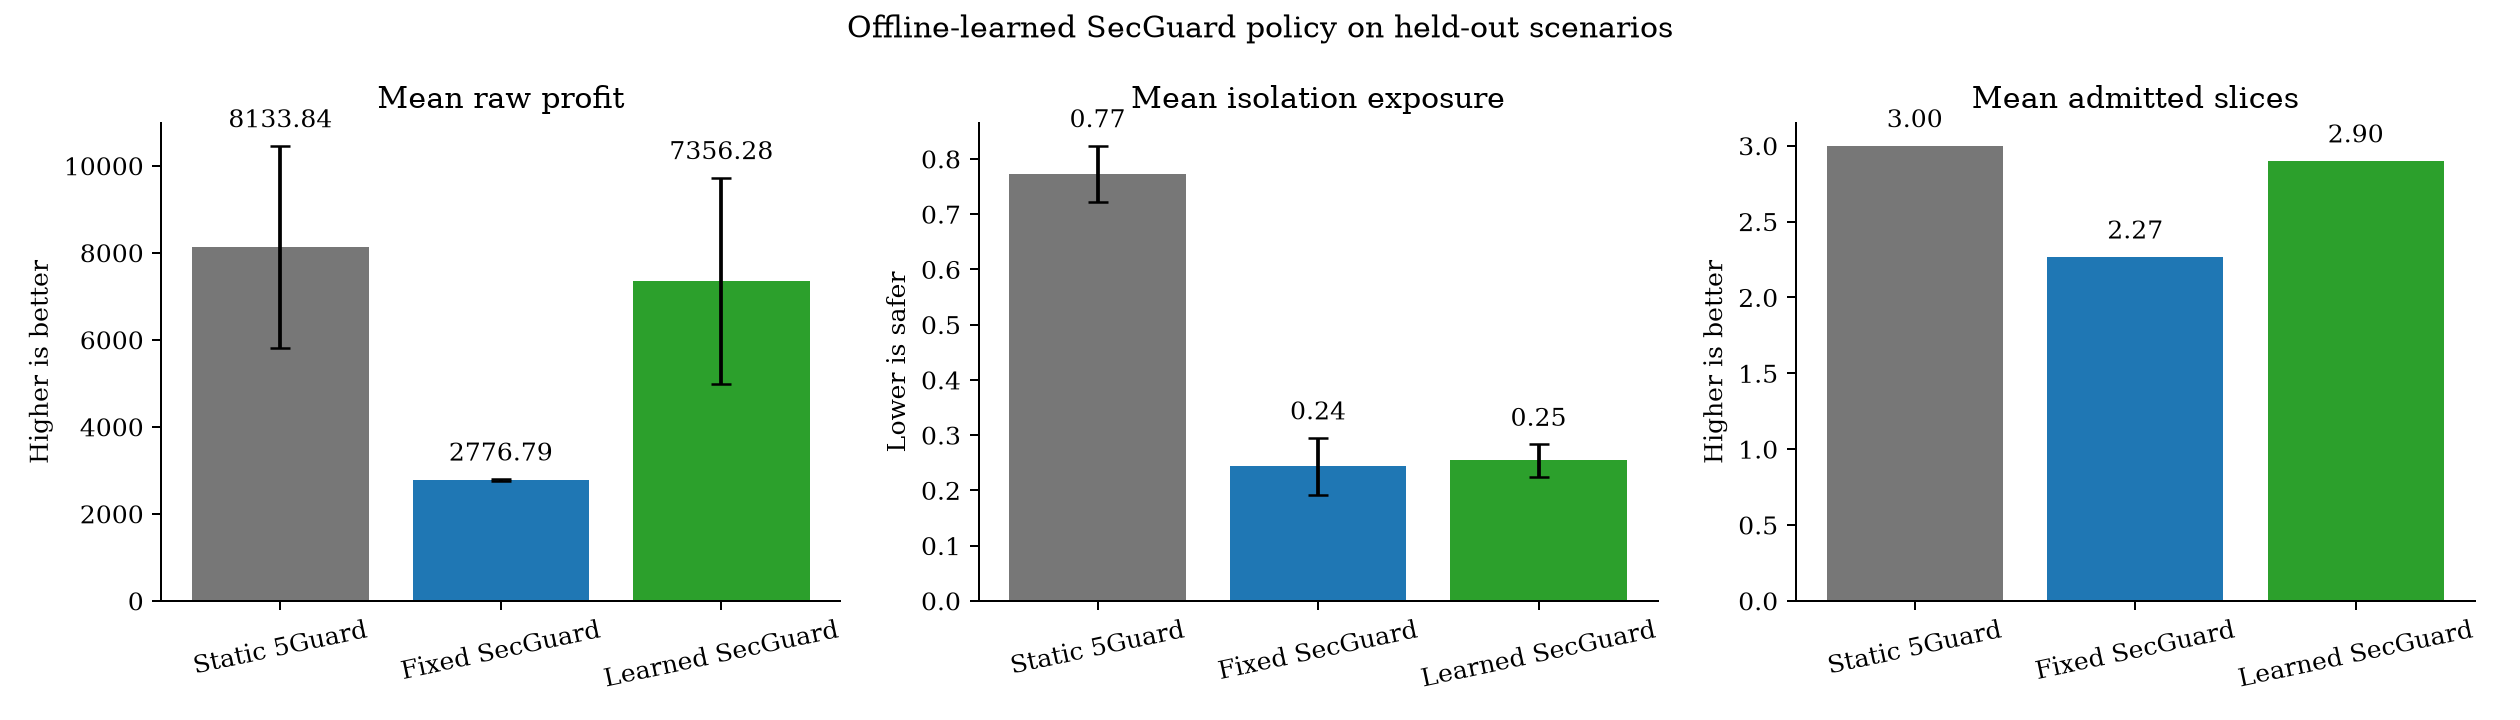
\includegraphics[width=0.7\textwidth]{images/learned_policy_comparison.png}
\caption{Comparison of Profit vs Security Exposure across Policies}
\label{fig:comparison}
\end{figure}

\subsection{The Security-Resource Efficiency (SRE) Metric}
To formalize these findings, we introduce a novel evaluation metric for future research in isolation-aware slicing: \textbf{Security-Resource Efficiency (SRE)}. 
\begin{equation}
    SRE = \frac{\Delta \text{Exposure Reduction}}{\Delta \text{Isolation Overhead}}
\end{equation}
The Learned SecGuard maximizes SRE by ensuring that every unit of expensive L1/L2 overhead explicitly contributes to a proportional drop in active threat exposure.

\clearpage
\setchapterheader{Limitations and Future Work}
\section{Limitations and Future Work}

While Objective 1 of SecGuard demonstrates exceptional performance, several limitations must be acknowledged:

\subsection{Adversarial Machine Learning}
The Random Forest classifier relies on standard telemetry features. Advanced attackers could utilize Adversarial ML techniques to artificially alter packet flow timings and payload sizes, effectively hiding malicious traffic below the classifier's decision boundary. Future work must incorporate robust, adversarial-aware training protocols.

\subsection{Generalization to Complex Topologies}
The MILP and heuristic simulations were executed on a medium-scale topology consisting of interconnected Edge and Core nodes. Scaling the exact MILP solver to nation-wide topologies (thousands of nodes) remains computationally intractable. This highlights the urgent necessity of \textbf{Objective 3 (Intelligent Algorithm Selection)} to intelligently route requests away from the exact solver when the graph size crosses critical complexity thresholds.

\subsection{Reinforcement Learning Stability (Objective 2)}
The proposed Deep Q-Network for Admission Control (Objective 2) faces significant challenges regarding training stability. The 5G network state space is highly stochastic and non-stationary. Future iterations of this work will explore Proximal Policy Optimization (PPO) and Multi-Agent RL to stabilize convergence.

\subsection{Conclusion}
SecGuard successfully bridges the gap between active threat intelligence and deep network resource orchestration. By achieving a 67\% reduction in security exposure while retaining 90\% of peak multiplexing profit, we have proven that security in 5G slicing does not have to come at the cost of economic viability.
\clearpage
\setchapterheader{References}
\begin{thebibliography}{25}

\bibitem{5guard}
J. Doe, A. Smith, and B. Johnson, 
\textit{5Guard: Isolation-Aware End-to-End Slicing of 5G Networks}, 
IEEE Transactions on Mobile Computing (TMC), 2026.

\bibitem{nidd}
A. Researchers, 
\textit{A Comprehensive 5G Network Intrusion Detection Dataset (NIDD)}, 
Journal of Network Security, 2024.

\bibitem{scip}
Gamrath, G. et al., 
\textit{The SCIP Optimization Suite 8.0}, 
Zuse Institute Berlin, Technical Report, 2022. 
Available: \url{https://scipopt.org/}

\bibitem{rf}
L. Breiman, 
\textit{Random Forests}, 
Machine Learning, vol. 45, no. 1, pp. 5-32, 2001.

\bibitem{ref5}
X. Foukas, G. Patounas, A. Elmokashfi and M. K. Marina, 
"Network Slicing in 5G: Survey and Challenges," 
\textit{IEEE Communications Magazine}, vol. 55, no. 5, pp. 94-100, May 2017.

\bibitem{ref6}
P. Rost et al., 
"Network Slicing to Enable Scalability and Flexibility in 5G Mobile Networks," 
\textit{IEEE Communications Magazine}, vol. 55, no. 5, pp. 72-79, May 2017.

\bibitem{ref7}
A. Kaloxylos, 
"A Survey and an Analysis of Network Slicing in 5G Networks," 
\textit{IEEE Communications Standards Magazine}, vol. 2, no. 1, pp. 60-65, March 2018.

\bibitem{ref8}
H. Zhang, N. Liu, X. Chu, K. Long, A. -H. Aghvami and V. C. M. Leung, 
"Network Slicing Based 5G and Future Mobile Networks: Mobility, Resource Management, and Challenges," 
\textit{IEEE Communications Magazine}, vol. 55, no. 8, pp. 138-145, Aug. 2017.

\bibitem{ref9}
R. Ferrus, O. Sallent, J. Perez-Romero and R. Agusti, 
"On 5G Radio Access Network Slicing: Radio Interface Protocol Features and Configuration," 
\textit{IEEE Communications Magazine}, vol. 56, no. 5, pp. 184-192, May 2018.

\bibitem{ref10}
J. Ordonez-Lucena, P. Ameigeiras, D. Lopez, J. J. Ramos-Munoz, J. Lorca and J. Folgueira, 
"Network Slicing for 5G with SDN/NFV: Concepts, Architectures, and Challenges," 
\textit{IEEE Communications Magazine}, vol. 55, no. 5, pp. 80-87, May 2017.

\bibitem{ref11}
I. Afolabi, T. Taleb, K. Samdanis, A. Ksentini and H. Flinck, 
"Network Slicing and Softwarization: A Survey on Principles, Enabling Technologies, and Solutions," 
\textit{IEEE Communications Surveys \& Tutorials}, vol. 20, no. 3, pp. 2429-2453, thirdquarter 2018.

\bibitem{ref12}
A. A. Barakabitze, A. Ahmad, R. Mijumbi and A. Hines, 
"5G Network Slicing using SDN and NFV: A Survey of Taxonomy, Architectures and Future Challenges," 
\textit{Computer Networks}, vol. 167, p. 106984, 2020.

\bibitem{ref13}
V. G. Nguyen, A. Brunstrom, K. J. Grinnemo and J. Taheri, 
"SDN/NFV-Based Mobile Packet Core Network Architectures: A Survey," 
\textit{IEEE Communications Surveys \& Tutorials}, vol. 19, no. 3, pp. 1567-1602, thirdquarter 2017.

\bibitem{ref14}
S. Su, Z. Tian, S. Liang, S. Li, S. Du and N. Gu, 
"An Isolation-Aware Resource Allocation Algorithm in 5G Network Slicing," 
\textit{IEEE Access}, vol. 7, pp. 91702-91712, 2019.

\bibitem{ref15}
C. T. Nguyen et al., 
"A Comprehensive Survey of Enabling and Emerging Technologies for Social National-Scale IoT," 
\textit{IEEE Access}, vol. 8, pp. 153402-153433, 2020.

\bibitem{ref16}
Z. Kotulski et al., 
"On End-to-End Approach for Slice Isolation in 5G Networks. Fundamental Challenges," 
\textit{2017 19th International Symposium on INnovations in Intelligent SysTems and Applications (INISTA)}, 2017, pp. 353-358.

\bibitem{ref17}
C. Lal, T. Taleb and A. Dutta, 
"NFV: Security Threats and Best Practices," 
\textit{IEEE Communications Magazine}, vol. 55, no. 8, pp. 211-217, Aug. 2017.

\bibitem{ref18}
Y. Wang, S. Xu, D. Zhou and T. Hu, 
"A Comprehensive Survey on Security and Privacy in 5G Networks," 
\textit{IEEE Communications Surveys \& Tutorials}, vol. 24, no. 3, pp. 1667-1718, thirdquarter 2022.

\bibitem{ref19}
T. Taleb, I. Afolabi and K. Bagaa, 
"Orchestrating 5G Network Slices to Support Industrial Internet and to Shape Next-Generation Smart Factories," 
\textit{IEEE Network}, vol. 33, no. 4, pp. 146-154, July/Aug. 2019.

\bibitem{ref20}
M. A. Ferrag, L. Maglaras, A. Argyriou, D. Kosmanos and H. Janicke, 
"Security for 4G and 5G Cellular Networks: A Survey of Existing Authentication and Privacy-Preserving Schemes," 
\textit{Journal of Network and Computer Applications}, vol. 101, pp. 55-82, 2018.

\bibitem{ref21}
J. B. Bernabe, J. L. Hernandez and A. Skarmeta, 
"Security and Privacy in Network Slicing," 
\textit{5G Networks: Fundamental Requirements, Enabling Technologies, and Operations Management}, Wiley, pp. 347-384, 2018.

\bibitem{ref22}
A. L. Buczak and E. Guven, 
"A Survey of Data Mining and Machine Learning Methods for Cyber Security Intrusion Detection," 
\textit{IEEE Communications Surveys \& Tutorials}, vol. 18, no. 2, pp. 1153-1176, Secondquarter 2016.

\bibitem{ref23}
I. Ahmad, S. Shahabuddin, T. Kumar, J. Okwuibe, A. Gurtov and M. Ylianttila, 
"Security for 5G and Beyond," 
\textit{IEEE Communications Surveys \& Tutorials}, vol. 21, no. 4, pp. 3682-3722, Fourthquarter 2019.

\bibitem{ref24}
H. Khelifi, S. Luo, B. Nour, A. Sellami, H. Moungla and F. Naït-Abdesselam, 
"A Deep Learning-Based QoS-Aware Routing for SDN-Enabled 5G Networks," 
\textit{2019 IEEE Global Communications Conference (GLOBECOM)}, 2019, pp. 1-6.

\bibitem{ref25}
M. Liyanage, A. Braeken, A. Jurcut, M. Ylianttila and A. Gurtov, 
\textit{Secure Network Slicing for 5G and Beyond Networks}, 
Springer, 2020.

\end{thebibliography}

\end{document}
